\documentclass[]{achemso}

\usepackage{graphicx}                   % Display figures using \includegraphics
\graphicspath{{../figures/}}            % Location for figures relative to .tex file path


\title{Supplementary Information for:  Methods for comparing uncertainty quantifications for material property predictions}
\author{Kevin Tran}
\affiliation{Chemical Engineering Department, Carnegie Mellon University, Pittsburgh, PA 15217}
\altaffiliation{These authors contributed equally to this work}
\author{Willie Neiswanger}
\affiliation{Machine Learning Department, Carnegie Mellon University, Pittsburgh, PA 15217}
\altaffiliation{These authors contributed equally to this work}
\author{Junwoong Yoon}
\affiliation{Chemical Engineering Department, Carnegie Mellon University, Pittsburgh, PA 15217}
\author{Qingyang Zhang}
\affiliation{Chemical Engineering Department, Carnegie Mellon University, Pittsburgh, PA 15217}
\author{Eric Xing}
\affiliation{Machine Learning Department, Carnegie Mellon University, Pittsburgh, PA 15217}
\author{Zachary W. Ulissi}
\affiliation{Chemical Engineering Department, Carnegie Mellon University, Pittsburgh, PA 15217}
\email{zulissi@andrew.cmu.edu}


\begin{document}

Figure~\ref{fig:resids} shows how the residuals of each model are correlated with each other.
All pairs of models show a positive correlation between each other.
This suggests that poor predictions made by one model were also made by most other models, qualitatively speaking.
This observation is consistent with the finding that the accuracy of all models in this study were comparable.
No single model was substantially better at predicting the outlying points than any other model.

\begin{figure}
    \centering
    \includegraphics[width=\textwidth]{corners/residual_correlations.pdf}
    \caption{Corner plot of the residuals of all models.
        Each subfigure shows the parity between the residuals of pairs of models.
        Solid contour lines delineate quartiles of the point distribution.
        Single, faded points indicate parity points in the fourth, least dense quartile of points.
        Shaded pixels indicate the highest density of points with darker shading indicating a higher density.
        The figures along the diagonal show histogram distributions of the residuals for each model.
        All units are in eV.
        }\label{fig:resids}
\end{figure}

Figure~\ref{fig:stdevs} shows how the predicted uncertainties of each model are correlated with each other.
The only pattern we could discern was the correlation between the GP and GP$_{NN-\mu}$ methods.
This correlation likely due to the fact that both methods used the same exact feature space for their GPs.
The only difference between the two were their mean functions.

\begin{figure}
    \centering
    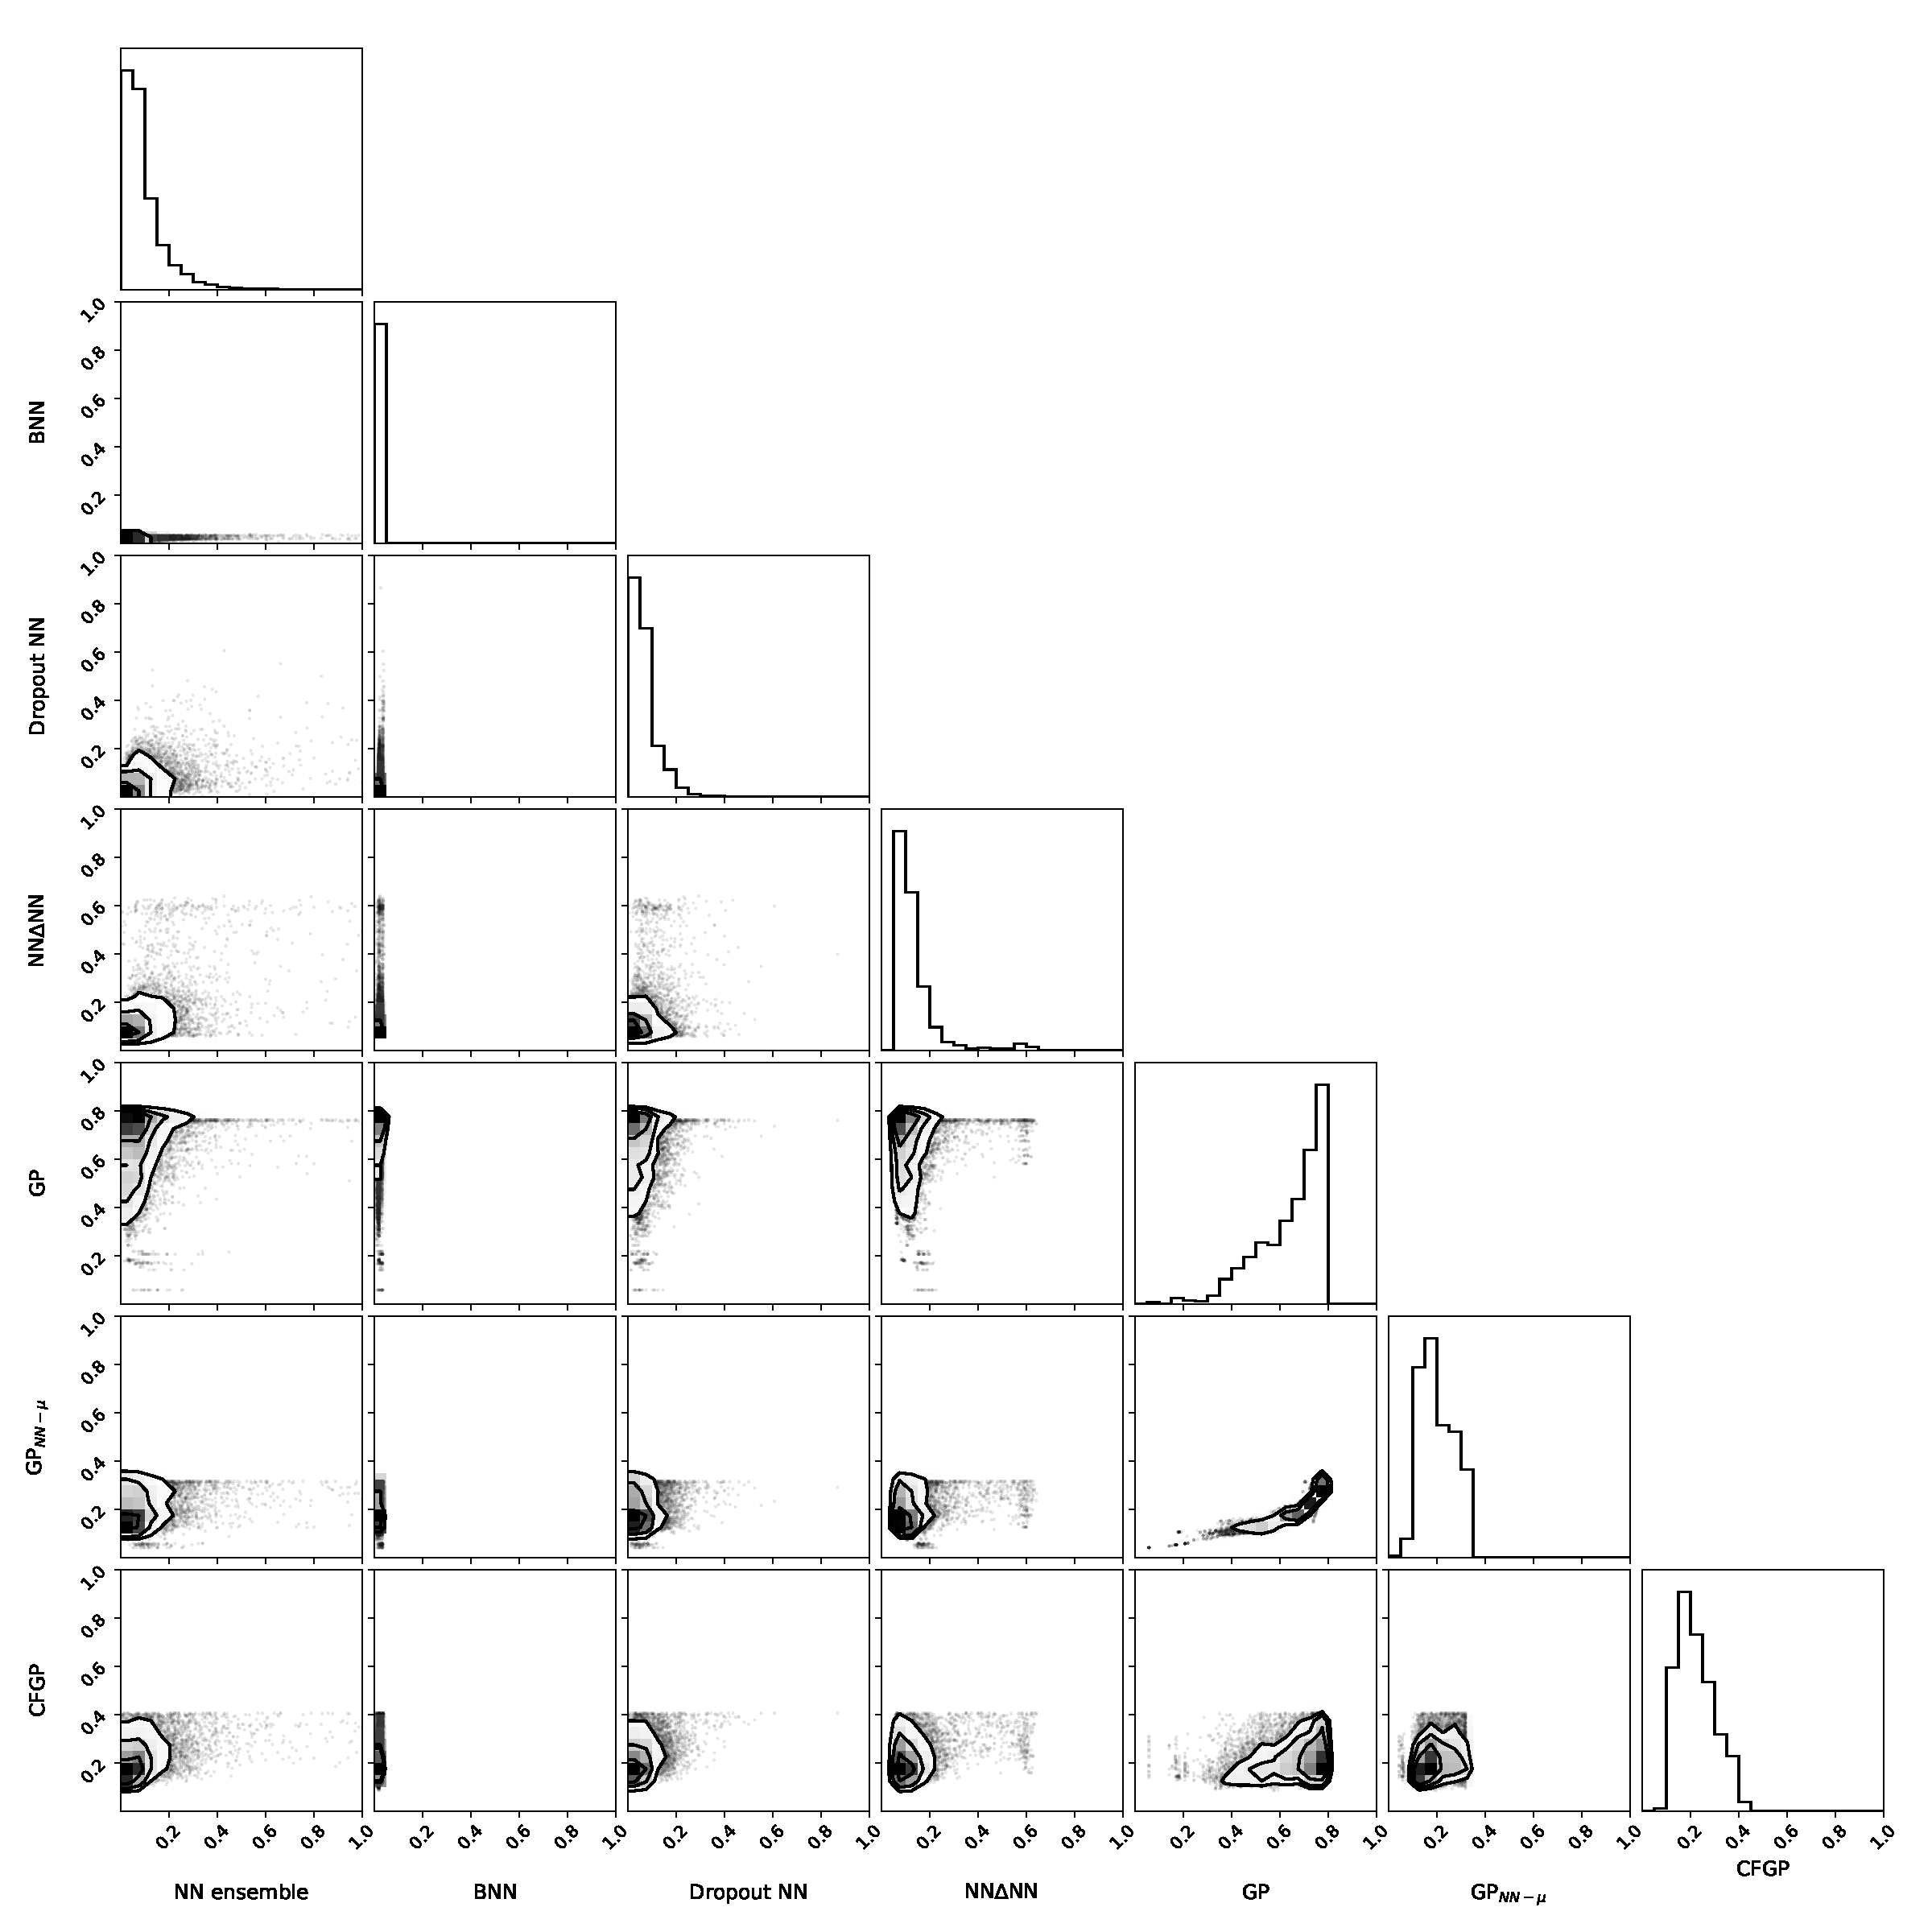
\includegraphics[width=\textwidth]{corners/stdev_correlations.pdf}
    \caption{Corner plot of the residuals of all models.
        Each subfigure shows the parity between the estimated standard deviations of pairs of models.
        Solid contour lines delineate quartiles of the point distribution.
        Single, faded points indicate parity points in the fourth, least dense quartile of points.
        Shaded pixels indicate the highest density of points with darker shading indicating a higher density.
        The figures along the diagonal show histogram distributions of the predicted standard deviations for each model.
        All units are in eV.
        }\label{fig:stdevs}
\end{figure}

\end{document}
